%%% 3Background / %%%
\chapter{Background} \label{ch:background}
%provide overview of topic that might be unfamiliar to 
%the readers
\section{Reputation algorithms} \label{sec:sectionlabel}
\subsection{Graph properties}
A graph, as the name suggests can be used to represent objects and their relationships 
graphically. A graph G is an ordered triple (V,E,$\varphi$$_{G}$) where V is a non empty set
of vertices v, E is a non empty set of edges e that connects two vertices and 
$v \in V, e \in E$. $\varphi$$_{G}$ is an incidence function that assigns pair of vertices
to each edge of the graph G. $\varphi$$_{G}$(e) = uv represents that e is an edge that 
joins vertices u and v. Graph properties can be leveraged to represent an interaction 
graph of network for reputation system. Each node on the network, v can represent 
individuals and the edges that connect the nodes can represent the relationships 
between those nodes. The edge can have varying weights to represent the strength of 
relationship between the nodes. \cite{bondy1976graph}
%cite graph theories and applications:
%http://citeseerx.ist.psu.edu/viewdoc/download?doi=10.1.1.721.3161&rep=rep1&type=pdf
%more concept based on what is needed to know when representing/modeling the network.

\subsection{EigenTrust}
EigenTrust is a reputation management algorithm for P2P network that aims to minimize 
malicious behaviour in the network and is based on the notion of transitive trust.
i.e. If a peer \textit{i} trusts a peer \textit{j} then all other peers trusted by 
\textit{j} is also trusted by \textit{i}. 
In EigenTrust, global reputation of each peer \textit{i} is given by local trust value 
assigned to peer \textit{i} by other peers and is weighted by the global reputation 
of assigning peers. 
A local trust value $s_{ij}$ is calculated by 
each peer \textit{i} which represents the opinion \textit{i} has of \textit{j}. $s_{ij}$
is the difference of satisfactory and unsatisfactory transactions peer \textit{i} had 
with other peers \textit{j}.
\begin{equation}
	s_{ij} = sat(i,j) - unsat(i,j) \\ 
\end{equation}
where sat(i,j) represents number of satisfactory transactions that \textit{i} had with 
\textit{j} whereas unsat(i,j) represents number of unsatisfactory transactions. \\
To prevent malicious peers from assigning arbitrarily high local trust values to 
other malicious peers, the local trust value is normalized as $c_{ij}$ before aggregating 
them. 
\begin{equation}
	c_{ij} = \frac{max(s_{ij},0)}{\sum_{j}max(s_{ij},0)}
\end{equation}
$C_{ij}$ keeps changing depending on the good or bad interaction between peer \textit{i} 
and peer \textit{j}.
Based on the local trust value assigned by other peers, each peer has a global trust 
value that determines their standing in the network. To aggregate the normalized local 
trust values, the approach used is friend-friend reference where a peer \textit{i} 
would ask its acquaintances about their opinion about other peers. Trust that 
peer \textit{i} places in peer \textit{k} by asking his friends can be denoted by 
$t_{ik}$ as : 
\begin{equation}
	t_{ik} = \sum_{j} c_{ij} c_{jk}
\end{equation}
Each peer asks other peers about their opinion which is weighted based on how much peer 
\textit{i} trusts them. 
If we define C as a matrix $[c_{ij}]$ and $t_{i}$ as a vector containing values 
$t_{ik}$, then $t_{ik}$ = $C^T\vec{c_{i}}$. This helps a peer get a wider view of 
the network more than its own experience. This can continue for many nodes until peer 
\textit{i} asks his friend's friend's and friend's friend can be consulted further to 
receive a broader view of the network. For \textit{n} nodes, we can represent \textit{t}
as t = $(C^T)^n c_{i}$. For a large enough value of \textit{n} , trust vector 
$\vec{t_{i}}$ will converge to same vector for every peer \textit{i} and could give 
complete view of the network. 
\textit{t} is the global trust vector where $t_{j}$ quantifies the trust system places in 
peer \textit{j}. 
EigenTrust is robust to malicious peers and good for decreasing inauthentic file downloads 
in a P2P network. However, it doesn't address the issues such as inactive peers, where a 
peer doesn't download from anywhere else, malicious collectiveness, where malicious peers 
collude to inflate the trust value. It also doesn't have a way to calculate negative trust 
and is entirely based on user feedback. \cite{kamvar2003eigentrust}

% The approach used for deriving these 
% values are past history and friend-friend reference. 

%cite: http://ilpubs.stanford.edu:8090/562/1/2002-56.pdf
%cite: https://www.cs.indiana.edu/~kapadia/courses/I590-Fall-09/internal/eigentrust.pdf

\subsection{Net flow Rate convergence}
Net flow rate convergence can help to determine anomaly in the network. By looking at how 
fast the net flow converges to zero, it can detect unusual behaviour in the network. 
The flow in a network can be measured by looking at inflow and outflow edges and 
calculating their differences. Inflow edges are all incoming edges in the graph and 
outflow edges are all outgoing edges . (diagram) Net flow convergence rate is the rate at which the net flow converges to the global net flow which is zero. 
Depending upon how fast the net flow in a graph converges to zero, it can be useful to 
detect anomaly.(example diagram) 

%cite: Decentralized Reputation system for transaction network. 
%Net flow convergence is used by (cite) and seems useful in detecting sybil node. 

\subsection{Binomial Random Walk}

\section{Cryptography}
\subsection{Basic Concepts}
Cryptography offers algorithms to achieve confidentiality, integrity, authenticity 
and non repudiation. Confidentiality and integrity ensures that the information 
being communicated is not disclosed or has been modified to or by any unauthorized 
parties. The data is hidden or encrypted such that only the authorized parties can 
make sense out of it i.e. decrypt using the previously agreed upon key. 
An illustration of 
sending encrypted messages that can only be decrypted with the shared key is presented 
in figure ~\ref{fig:basic terminology}
\begin{figure}[h]
\centering
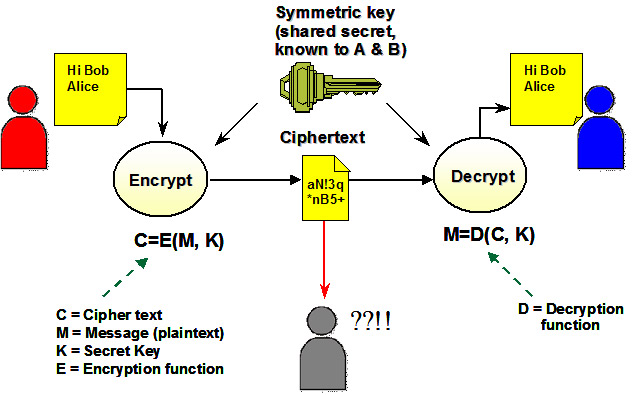
\includegraphics[width = 1.0\textwidth]{symmetric-alice-bob.jpg}
\caption{Symmetric Key in use \cite{symmetrickey} }
\label{fig:basic terminology}
\end{figure}
%cite : http://securitycerts.org/review/symmetric-key-in-use.htm
Authenticity and non repudiation are another properties that makes sure that 
the sender is who he claims to be and that the sender cannot deny having sent 
the message. For these properties, symmetric key cryptography wouldn't be 
enough. This is where Asymmetrical cryptography or public key cryptography comes 
in which uses key pairs, private key known only to the owner and public key that 
can be distributed publicly. Public key verifies the holder of the private key 
and encryption of message. This encrypted message can only be decrypted by that 
paired private key. One of the major application of public key cryptography is 
Digital Signatures, described in more detail in section (Blockchain section ..) 
which is useful in preserving the properties of authenticity and non 
repudiation. 

A cryptosystem can be seen as a five tuple (P,C,K,E,D) that satisfies the following
conditions: \\ 
P is a finite set of plain texts.  \\
C is a finite set of cipher texts. \\ 
K, 	the keyspace is a finite set of keys \\
E, set of encryption rules $e_k$: P $\Rightarrow$ C \\
D, sete of decrytion rules $d_k$ : C $\Rightarrow$ M. \\
for each k $\in$ K, there is $e_{k}$ $\in$ E and $d_{k} \in$ D such that 
$d_{k}(e_{k}(m))$ = m for every plaintext m $\in$ P. \\

% A cryptosystem shouldn't rely on the privacy of algorithm used to secure the system. 
% According to Kerckhoff's principle, a cryptosystem should be secure even if everything 
% about the system, except the key, is public knowledge. Another encryption method 
% known as public key cryptography makes use of two different keys for encryption 
% and decryption respectively. It uses public key and private key pairs that are related 
% but is hard to deduce one from the other. When sending a message, one might make public 
% the public key to the whole network but the private key must not be known/shared with 
% anyone but the owner himself. 
%Diffie-Hellman key exchange
%encryption, decryption 

\subsection{Hash functions}
Cryptographic hash functions are one way function, also known as mathematical trap door function that transforms an input message into a fixed length binary output. It 
is one way because although transforming a message input to a hash value or a message 
digest can be done in constant time, reversing the operation is practically 
impossible to achieve as its computationally inefficient. 
Earlier hash functions include 
MD5 which produces a 128 bit hash value but is vulnerable and can be cracked by brute 
force attack. The predecessors hash functions are sha-256 preceeded by sha-1, sha-2
and others. 
Their applications include digital signature, message authentication both of 
which are interesting for blockchain as will be discussed in section(name). The
important characteristics of hash functions are their deterministic output, meaning
given a fixed input, it will always generate the same output. It offers collision 
resistant property i.e. it is 
impossible or extremely rare to get the same hash value for two different messages. 
If m1 and m2 are the message and h(m1) and h(m2) are hash functions applied to them 
respectively, collision resistant ensures that h(m1) != h(m2). 
Another important characteristic of hash function is that the hash value provides no 
indication of the original information that was hashed thus making it efficient for 
hiding information. 

%deterministic output 
%computationally efficient
%hash collision: collision resistant h(m1) != h(m2)
%hide information
%sha-1, sha-2, sha-256 

\subsection{Digital Signature}
%public key , private key, sign message, verify 
Digital signatures 
%RSA
%Sign with private key, verify with public key

% \subsection{Proof-Of-Work}
% solve a computationally expensive problem and show a proof before being able to do 
% something on the network. 

\section{Blockchain Technology}
\subsection{Basic Concepts}
transaction, message, signature, broadcast, verify, network, miners, validate, write blocks 

\subsection{Evolution \& Categories}
Bitcoin,Ethereum, private permissioned
\subsection{Consensus algorithms}
proof of work, proof of stake, proof of validatioin, proof of authority, and others


\subsection{Smart contracts}
define,explain
\subsection{Applications}




